\section{Обработка табличных данных. Часть 1.}

\textbf{Задание:} Найти сумму нечетных элементов, меньших заданного числа. 
Вывести максимальный четный элемент. 

Создано окно приложения, содержащее два элемента TextBox, два элемента Label, 4 элемента Button, и 1 элемент DataGridView. 
Для отображения сообщений об ошибках в окно добавлен элемент ErrorProvider. Вид окна представлен на рисунке \ref{fig:task4_form}.

\begin{figure}[H]
    \centering
    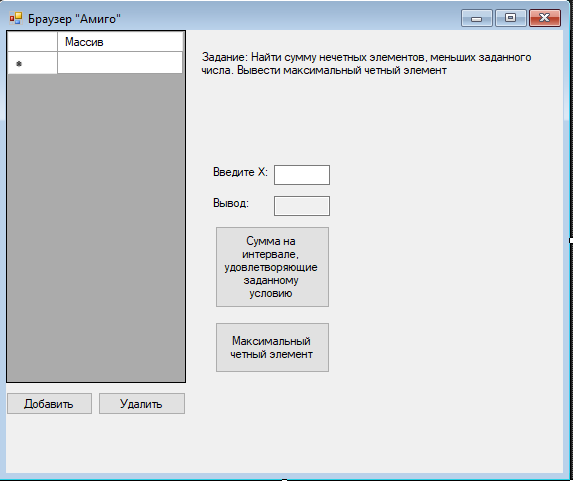
\includegraphics{task4/form.png}
    \caption{Внешний вид формы программы}
    \label{fig:task4_form}
\end{figure}

У элементов изменены значения некоторых атрибутов. 
Значения измененных атрибутов представлены в таблице \ref{table:params2}.

\begin{table}[H]
    \small
    \caption{Значения атрибутов элементов в приложении <<Обработка табличных данных. Часть 1.>>}\label{tab:fact-attr}
    \begin{tabular}{|l|l|}\hline
    Наименование атрибута & Значение\cr\hline
    \multicolumn{2}{|l|}{Для формы}\cr\hline
    \verb"Text" & \verb"Браузер "Амиго""\cr\hline
    \verb"FormBorderStyle" & \verb"FixedSingle"\cr\hline
    \verb"MaximizeBox" & \verb"False"\cr\hline
    \multicolumn{2}{|l|}{Для первой надписи}\cr\hline
    \verb"(Name)" & \verb"xLabel"\cr\hline
    \verb"Text" & \verb"Введите X"\cr\hline
    \multicolumn{2}{|l|}{Для второй надписи}\cr\hline
    \verb"(Name)" & \verb"lblOutput"\cr\hline
    \verb"Text" & \verb"Вывод"\cr\hline
    \multicolumn{2}{|l|}{Для первого текстового поля}\cr\hline
    \verb"(Name)" & \verb"txtX"\cr\hline
    \multicolumn{2}{|l|}{Для второго текстового поля}\cr\hline
    \verb"(Name)" & \verb"txtOutput"\cr\hline
    \multicolumn{2}{|l|}{Для кнопки суммирования}\cr\hline
    \verb"(Name)" & \verb"btnSummary"\cr\hline
    \verb"Text" & \verb"Сумма на интервале, удовлетворяющие заданному условию"\cr\hline
    \multicolumn{2}{|l|}{Для кнопки для нахождения максимального четного элемента}\cr\hline
    \verb"(Name)" & \verb"btnFindMaxEven"\cr\hline
    \verb"Text" & \verb"Максимальный четный элемент"\cr\hline
    \multicolumn{2}{|l|}{Для кнопки для нахождения максимального четного элемента}\cr\hline
    \verb"(Name)" & \verb"btnFindMaxEven"\cr\hline
    \verb"Text" & \verb"Максимальный четный элемент"\cr\hline
    \multicolumn{2}{|l|}{Для кнопки добавления ряда}\cr\hline
    \verb"(Name)" & \verb"btnAdd"\cr\hline
    \verb"Text" & \verb"Добавить"\cr\hline
    \multicolumn{2}{|l|}{Для кнопки удаления ряда}\cr\hline
    \verb"(Name)" & \verb"btnRemove"\cr\hline
    \verb"Text" & \verb"Удалить"\cr\hline
    \multicolumn{2}{|l|}{Для таблицы}\cr\hline
    \verb"(Name)" & \verb"grid"\cr\hline
    \verb"(Name)" & \verb"grid"\cr\hline
    \multicolumn{2}{|l|}{Для обработчика ошибок}\cr\hline
    \verb"(Name)" & \verb"errorProvider1"\cr\hline
    \end{tabular}
    \label{table:params2}
\end{table}

Для изменения количества рядов в таблице были реализованы кнопки добавления
и удаления ряда. Код соответствующих функций приведен ниже:

\begin{minted}[fontsize=\small, breaklines=true, style=bw, linenos]{cpp}
    private: System::Void btnAdd_Click(System::Object^ sender, System::EventArgs^ e) { // Добавление
			this->grid->Rows->Add(1);
	}
    private: System::Void btnRemove_Click(System::Object^ sender, System::EventArgs^ e) { // Удаление
		if (!this->grid->CurrentRow->IsNewRow) {
			int i = this->grid->CurrentRow->Index;
			this->grid->Rows->Remove(this->grid->Rows[i]);
		}
	}

\end{minted}

Решение каждой из двух задач реализовано в соответствующих кнопках. Код 
представлен ниже:

\begin{minted}[fontsize=\small, breaklines=true, style=bw, linenos]{cpp}
        private: System::Void btnSummary_Click(System::Object^ sender, System::EventArgs^ e) { // Вычисление необходимой суммы
			ClearOutput();
			bool noBadCells = true;
			bool check2 = true;
			if ((int)WrongCells->size() > 0) {
				noBadCells = false;
			}
			int xValue;
			bool isCorrectValue = Int32::TryParse(txtX->Text, xValue);
			if (!isCorrectValue) {
				errorProvider1->SetError(txtX, "Неверное значение для X");
			}
			if (!isCorrectValue) {
				return;
			}
			else {
				errorProvider1->SetError(txtX, String::Empty);
			}
			if (!noBadCells) {
				return;
			}
			int summary = 0;
			for (int i = 0; i < this->grid->RowCount; ++i) {
				int val = System::Convert::ToInt32(this->grid->Rows[i]->Cells[0]->Value);
				if (val % 2 == 1 && val < xValue) {
					summary += val;
				}

			}
			ClearOutput();
			txtOutput->Text = System::Convert::ToString(summary);
		}
		private: System::Void btnFindMaxEven_Click(System::Object^ sender, System::EventArgs^ e) { // Вывод необходимого максимального элемента на экран
			ClearOutput();
			if (WrongCells->size() > 0) {
				return;
			}
			int max_val = -1e9;
			int max_ind = -1;
			for (int i = 0; i < this->grid->RowCount; ++i) {
				int val = System::Convert::ToInt32(this->grid->Rows[i]->Cells[0]->Value);
				if (val > max_val && val % 2 == 0) {
					max_val = val;
					max_ind = i;
				}
			}
			ClearOutput();
			txtOutput->Text = System::Convert::ToString(max_val);
		}
\end{minted}

Контроль за корректностью введенных данных осуществляется через поддерживание
невалидных ячеек в set из библиотеки STL. Работа с ней осуществляется через 
обработку события CellLeave:

\begin{minted}[fontsize=\small, breaklines=true, style=bw, linenos]{cpp}
    private: System::Void grid_CellLeave(System::Object^ sender, System::Windows::Forms::DataGridViewCellEventArgs^ e) {
			int val = 0;

			System::String^ Value = System::Convert::ToString(this->grid->Rows[grid->CurrentRow->Index]->Cells[0]->EditedFormattedValue);
			
			bool isCorrectValue = Int32::TryParse(Value, val); // Пробуем записать в InputNumber число из потока
			if (!isCorrectValue && (Value != "" && grid->CurrentRow->Index != grid->RowCount)) {
				errorProvider1->SetError(grid, "Неверный тип для ячейки");
				WrongCells->insert(grid->CurrentRow->Index);
			}
			else {
				WrongCells->erase(grid->CurrentRow->Index);
				if ((int)WrongCells->size() == 0) {
					errorProvider1->SetError(grid, String::Empty);
				}
			}
			
		}
\end{minted}

После запуска приложения на экране появляется окно (см. рисунок \ref{fig:exec4})
\begin{figure}[H]
    \centering
    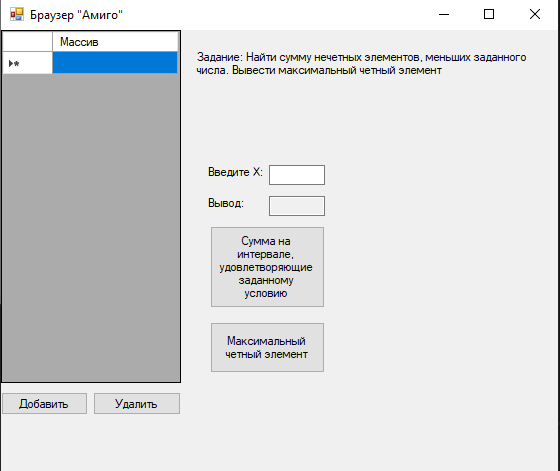
\includegraphics{task4/exec.png}
    \caption{Скриншот запуска программы}
    \label{fig:exec4}
\end{figure}

При вводе целого числа после нажатия кнопки в поле вывода приводится
результат вычисления суммы в заданном интервале (см. рисунок \ref{fig:result41}).
\begin{figure}[H]
    \centering
    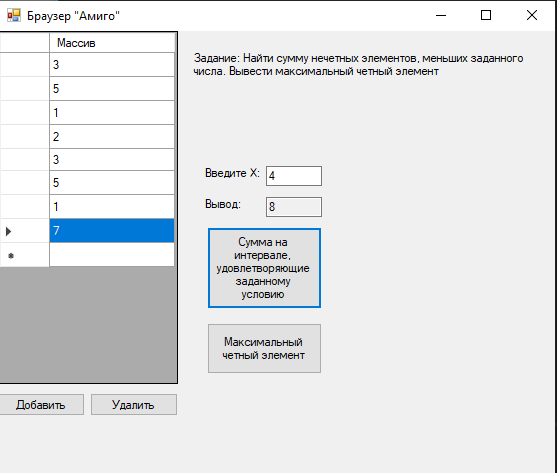
\includegraphics{task4/result1.png}
    \caption{Результат работы}
    \label{fig:result41}
\end{figure}

При вводе целого числа после нажатия кнопки в поле вывода приводится
результат вычисления максимального четного элемента (см. рисунок \ref{fig:result42}).
\begin{figure}[H]
    \centering
    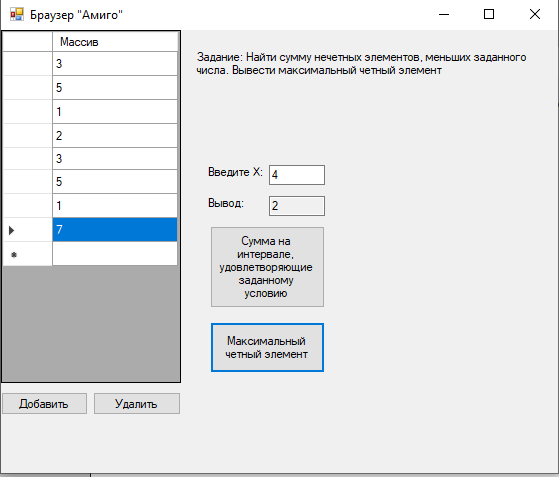
\includegraphics{task4/result2.png}
    \caption{Результат работы}
    \label{fig:result42}
\end{figure}

Ввод некорректных значений обрабатывается элементом \verb|errorProvider1| и 
сопровождается сообщением об ошибке (см. рисунок \ref{fig:error4} )
\begin{figure}[H]
    \centering
    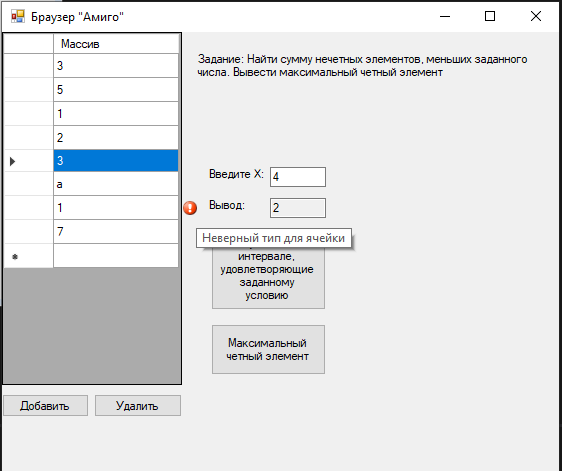
\includegraphics{task4/error.png}
    \caption{Сообщение об ошибке}
    \label{fig:error4}
\end{figure}
Полный код программы приведен в приложении А.